\newchapter{Introduction}{Introduction}{An Introduction to Self-interacting Dark Matter and Merging Galaxy Clusters}
\label{chapter:1}

\noindent Note if and where this material was published. \\

Chapter abstract text

%--------------------------------------------------------------------
\section{Standard Model of Cosmology}

contents of the Universe

see e.g. Bullock 2010 notes \citep{Bullock:2010uv}


%--------------------------------------------------------------------
\section{Dark Matter}

\subsection{Historical Review}

\subsection{General Properties of Dark Matter}

%--------------------------------------------------------------------
\section{Motivation for Studying Self-interacting Dark Matter}

\subsection{Early Motivation}

Despite the success of the CDM paradigm there are a number of recent observations which appear to be in conflict:

Earliest was the missing satellites problem \citep{Moore:1999ja} \citep{Klypin:1999ej}

	Motivated work of Spergel and Steinhardt into SIDM \citep{Spergel:2000cb}

	Recent work shows that doesn't SIDM doesn't significantly reduce the number of satellites

Has since become less of a problem (simulations and SDSS)

\subsection{Early SIDM Constraints}

Halo Shapes: Miralda-Escudé 2002

Cluster density core: Yoshidal et al. 2000

Dwarfs density cores: Dave et al. 2001

Subhalo evaporation: Gnedin \& Ostriker 2001

Merging Cluster: Randall et al 2008

Growth of SMBH: Hennawi \& Ostriker 2002

Moore et al. 2000 \citep{Moore:2000ee}

Problems with each of those (see presentation slides)

Recent revisions to these constraints \citep{Peter:2012vi}

\subsection{Recent Motivation}

Cusp-core problem

	rachael kuza de neray
	drew newman
	counter example: Tomasso's student, Louie Strigari (see KITP presentation)

Too-big to fail

\subsection{SIDM as a Solution}

How SIMD may resolve these problems

Narrow window of parameter space to probe \citep{Rocha:2012tr}

%--------------------------------------------------------------------
\section{Probes of SIDM}



Baryon degeneracy and why merging cluster may be the best probe

%--------------------------------------------------------------------
\section{Merging Galaxy Clusters as Probes of Self-Interacting Dark Matter}

Section text

\subsection{Merging Galaxy Clusters}

Think about moving some of the Figure \ref{fig:4ConstraintMethods} caption to the body text to make for a more concise caption.

\begin{figure}
\centering
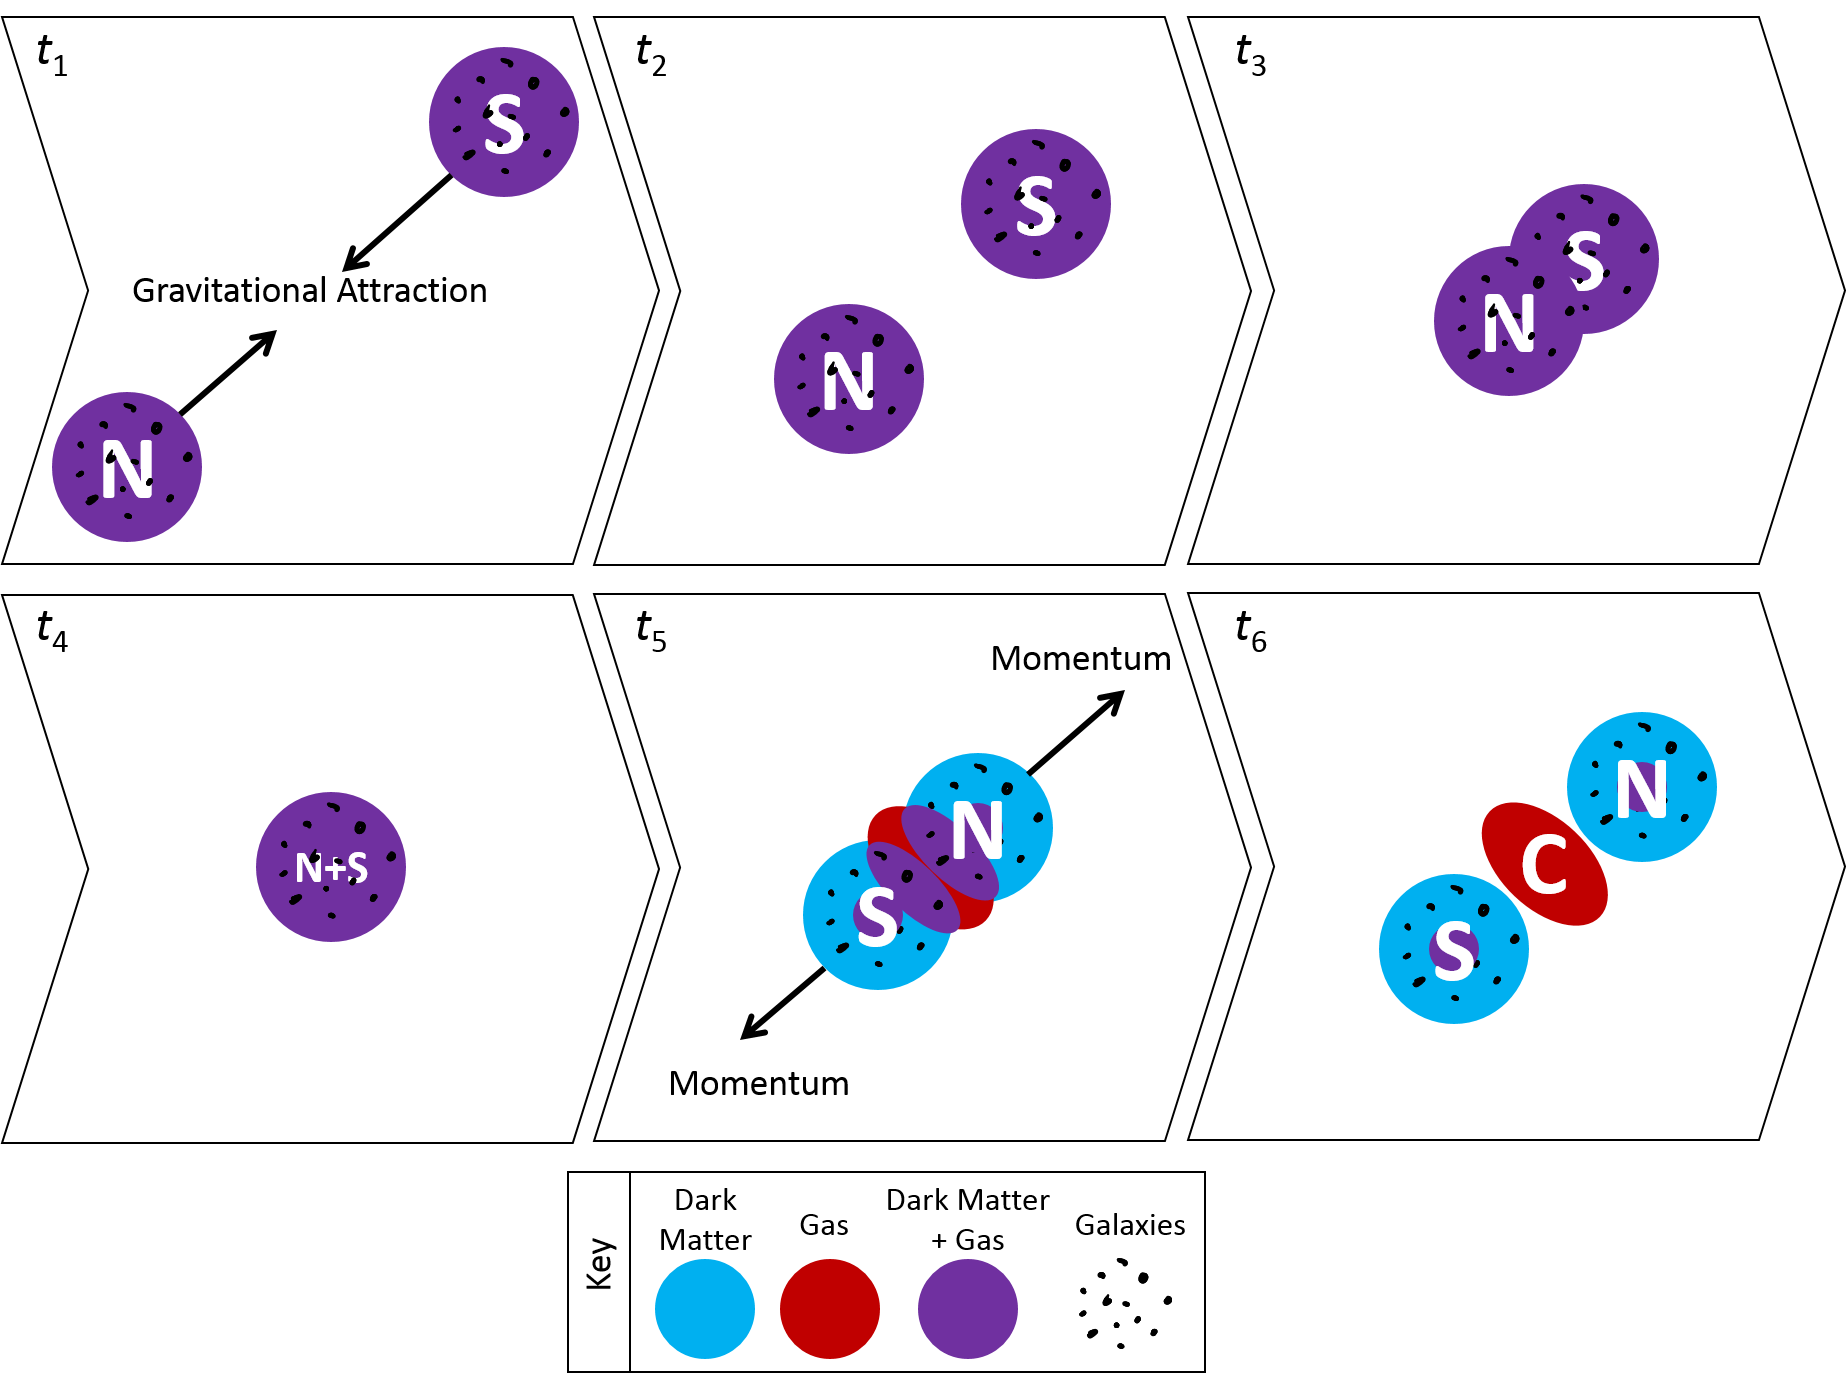
\includegraphics[width=6in]{Chapter1/MergerTimeSeries.png}
\caption{A basic time series leading to a dissociative galaxy cluster merger (assuming the Standard Model of Cosmology).
Two galaxy clusters (N \& S), each consisting of overlapping halos of DM and gas as well as sparsely populated galaxies, begin with an initial physical separation ($t_{\rm 1}$).
Due to the mass of each galaxy cluster they experience a gravitational attraction and accelerate towards one another until eventually they collide ($t_{\rm 1}$--$t_{\rm 4}$).
By convention time $t_{\rm 4}$ is defined as the ``collision''.
Because there is so much space between the galaxies, a strong interaction between any two galaxies is extremely unlikely and they can be treated as effectively collisionless particles.
And since the galaxies of each subcluster have built up momentum they will pass through and begin to separate (this time on the opposite side), $t_{\rm 5}$.
The gas however is more evenly distributed, thus an interaction between gas particles of each subcluster is more likely.
This interactions will convert some of the infall kinetic energy into thermal energy (i.e. the gas of each subcluster will experience ram pressure), the net effect being that the gas halo of each subcluster is slowed with respect to the galaxies and much of it becomes dissociated remains centered between the galaxies of the two subclusters ($t_{\rm 6}$ C).
Much like the galaxies the DM behaves in a nearly collisionless manner and appears largely coincident with the galaxies.
At $t_{\rm 6}$ the galaxy cluster merger is classed as \emph{dissociative merger}.
\label{fig:MergerTimeSeries}}
\end{figure}  

\subsection{Constraining Self-Interacting Dark Matter with Merging Galaxy Clusters}

Think about moving some of the Figure \ref{fig:4ConstraintMethods} caption to the body text to make for a more concise caption.

\begin{figure}
\centering
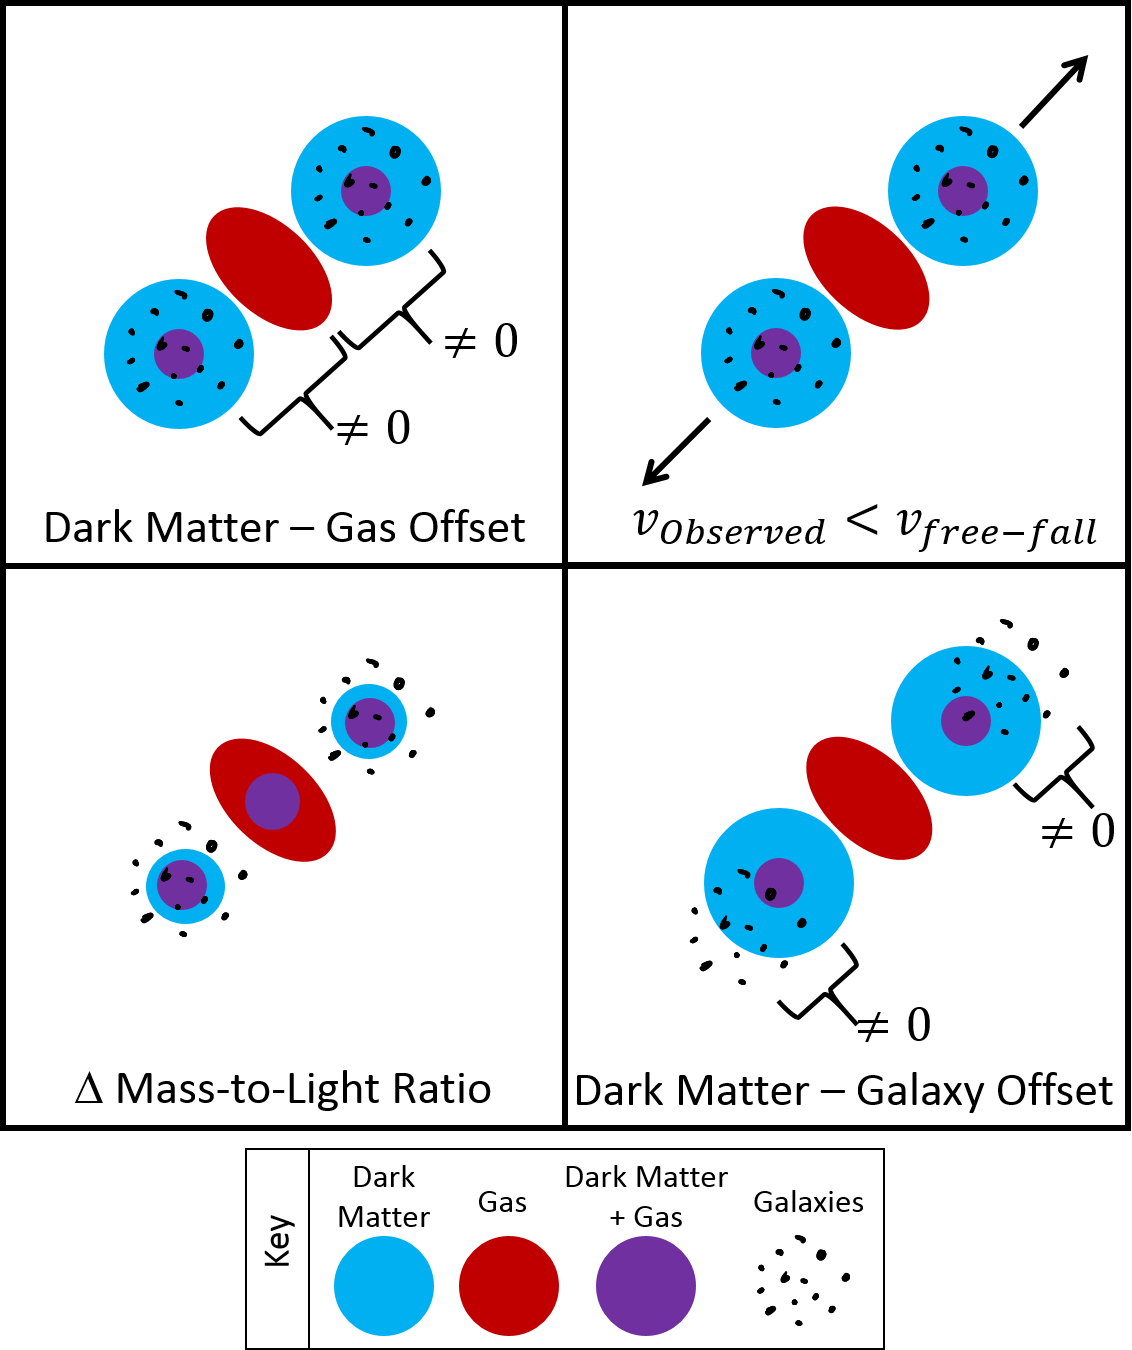
\includegraphics[width=4in]{Chapter1/4ConstraintMethods.png}
\caption{The four means of constraining $\sigma_{\rm SIDM}$ with merging clusters, originally outlined by \citet{Markevitch:2004dl} and \citet{Randall:2008hs}. 
\emph{Upper Left:} If the DM is significantly offset from the gas then the scattering depth of the dark matter ($\tau_{\rm DM}$) must be less than the scattering depth of the gas ($\tau_{\rm gas}$) and an upper limit can be placed on $\sigma_{\rm SIDM}$.
\emph{Upper Right:} If DM self-interacts during the merger, then the velocity of each subcluster will be slowed to some degree.
Thus if the observed velocity ($v_{\rm obs}$) is found to be consistent with the free-fall velocity ($v_{\rm free-fall}$) an upper limit can be placed on $\sigma_{\rm SIDM}$.
If however $v_{\rm obs}$ is significantly less than $v_{\rm free-fall}$, an upper limit could be potentially placed on $\sigma_{\rm SIDM}$.
\emph{Lower Left:} If DM self-interacts during the merger, then some fraction of the DM particles will scatter and become unbound from each subcluster.
Thus the mass-to-light ratio of each subcluster can be compared with the mass-to-light ratio of similar non-merging clusters, and depending on where the mass-to-light ratio of the merger is the same or less than the non-merging clusters' mass-to-light ratio, then respectively an upper limit or lower limit can be placed on $\sigma_{\rm SIDM}$.
\emph{Lower Right:} If the DM self-interacts during the merger, then the DM component of each subcluster will experience an additional drag force and will travel at a slower velocity than the respective subcluster galaxies.
Thus depending on whether a significant offset between the galaxies and DM is or is not observed, then respectively a lower limit or upper limit can be placed on $\sigma_{\rm SIDM}$.
\label{fig:4ConstraintMethods}}
\end{figure}  